Die Leerlaufspannung $U_{\text{0}}$ bezeichnet die Spannung, die ohne
fließenden Strom $I$ an der Spannungsquelle gemessen werden kann.
Sobald ein endlicher Strom fließt, sinkt die Spannung $U_{\text{k}}$ auf einen
Wert unterhalb $U_{\text{0}}$ ab. $U_{\text{K}}$ bezeichnet hierbei die
Klemmenspannung und fällt über der Spannungsquelle ab.
Der Spannungsabfall lässt sich durch den Innenwiderstand der Spannungsquelle
erklären.
Gemäß dem Zweiten Kirchhoffschen Gesetz
\begin{equation}
  \sum_\symup{n} \symup{U}_{0_\symup{n}} = \symup{\sum_m R_m I_m}
  \label{eqn:kirch}
\end{equation}
ist die Summer aller Leerlaufspannungen gleich der Summe aller
Spannungsabfälle an den Widerständen $\symup{R_m}$ der Masche.
Unter Berücksichtigung von
\begin{equation}
  U=R\cdot I
\end{equation}
gilt für Abbildung \ref{fig:real}_
\begin{equation}
  U_\symup{0}=I \cdot R_\symup{i} + I \cdot R_\symup{a}
  \text{bzw.}
  U_\symup{k}=I \cdot R_\symup{i} = U_\symup{0} - I \cdot R_\symup{a}
  \label{eqn:U0k}
\end{equation}
\begin{figure}[H]
  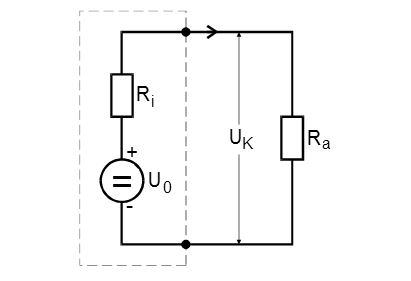
\includegraphics{bilder/real}
  \caption{Ersatzschaltbild einer realen Spannungsquelle mit Lastwiderstand
  $\symup{R_a}\cite{301}$}
  \label{fig:real}
\end{figure}
\\
Dabei ist $R_\symup{i}$ der Innenwiderstand der Stromquelle und $R_\symup{a}$
der Lastwiderstand im Stromkreis.
Der gestrichelt umrandete Teil von Abbildung \ref{fig:real} wird als
Ersatzschaltbild einer realen Spannungsquelle bezeichnet. Diese besteht aus
einer idealen Spannungsquelle und einem zugehörigen Innenwiderstand
$R_\symup{i}$.
